\documentclass[11pt,a4paper]{beamer}
\usetheme{Copenhagen}
\usepackage[latin1]{inputenc}
\usepackage{amsmath}
\usepackage{amsfonts}
\usepackage{amssymb}
\usepackage{graphicx}
\begin{document}
\section{Introduction}
\begin{frame}{Agenda}
\begin{block}{Agenda}
\begin{itemize}
\item Introduction \pause
\item Examples \pause
\item Optimization classes and usage
\end{itemize}
\end{block}
\end{frame}


\begin{frame}{Introduction}
\begin{block}{What is mathematical optimization}
Finding an optimal set of parameters $\textbf{x}$ which minimizes or maximizes an \textit{objective function} $f(\textbf{x})$, formally

\[ \hat{\textbf{x}} = \textnormal{arg} \underset{\textbf{x}}{\textnormal{min}} \hspace{5px} f(\textbf{x}) \]
\end{block}
\end{frame}
\begin{frame}{Visualisation}
\begin{figure}
\centering
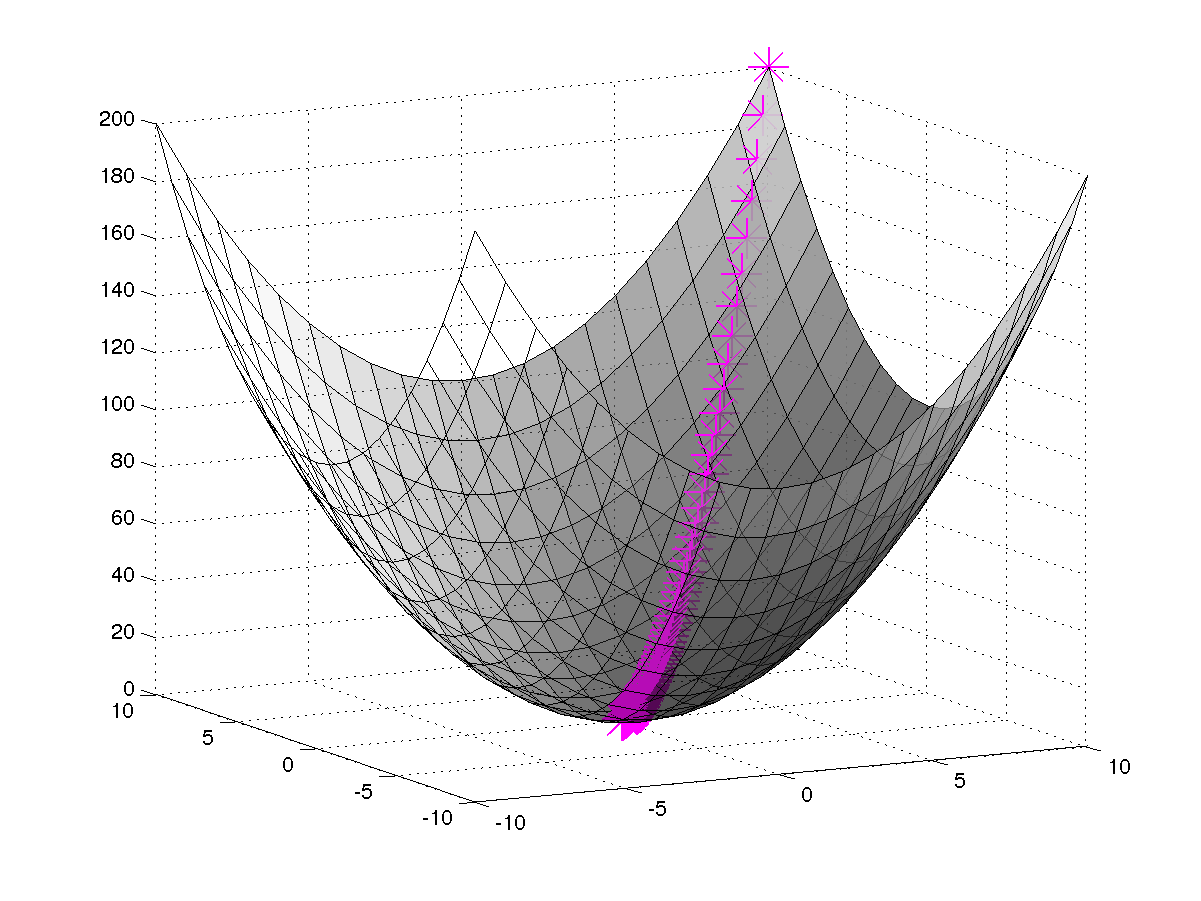
\includegraphics[width=0.7\linewidth]{images/gradientdescent}
\caption{Minimization of convex function, \textit{convex programming}}

\label{fig:gradientdescent}
\end{figure}
\end{frame}
\begin{frame}{How do we take advantage of it}
\begin{block}{Who cares about minima?} \pause
\begin{itemize}
\item Optimizing control systems \pause
\item Signal processing \pause
\item Statisticians (regression analysis) \pause
\item High frequency trading (maximize profits, minimize loss) \pause
\end{itemize}
\end{block}
\begin{block}{Why do we care about it?}
Many things are very easily perceived and processed by the human brain, but very difficult to have a computer to reason about. \pause
\begin{itemize}
\item Pattern recognition \pause
\item Face detection/recognition \pause
\item etc. etc. etc. 
\end{itemize}
\end{block}

\end{frame}

\begin{block}{Examples}

content...
\end{block}

\begin{frame}{Common problems}
\begin{block}{Important classes}
\begin{itemize}
\item Gradient descent algorithms (Newton)
\item Direct search algorithms
\item Evolutionary strategies
\end{itemize}
\end{block}


\end{frame}
\end{document}